\section{Quadratic Unconstrained Binary Optimization}\label{sec:algoritmi}

I problemi Quadratic Unconstrained Binary Optimization (QUBO) rappresentano una 
classe fondamentale di problemi di ottimizzazione in cui si cerca di minimizzare 
(o massimizzare) una funzione quadratica con variabili binarie, cioè variabili 
che possono assumere solo i valori 0 o 1. Ciò che rende i QUBO particolarmente 
interessanti è il fatto che molti problemi complessi di ottimizzazione possono 
essere riformulati in questo formato.

La caratteristica principale dei QUBO è la loro semplicità strutturale: sono 
problemi non vincolati, il che significa che l'unico vincolo è la natura binaria 
delle variabili. Nonostante questa apparente semplicità, i QUBO sono problemi 
NP-completi, il che significa che sono computazionalmente difficili da risolvere 
con metodi classici quando la dimensione del problema cresce.

L'importanza dei QUBO nel contesto del calcolo quantistico deriva dalla loro 
versatilità. Infatti, possiamo utilizzarli per risolvere una vasta gamma di 
problemi pratici come:

\begin{itemize}
    \item la colorazione dei grafi, dove si cerca di assegnare colori a nodi di 
        un grafo in modo che nodi adiacenti abbiano colori diversi;
    \item il partizionamento di numeri, dove si cerca di dividere un insieme di 
        numeri in gruppi con somma simile;
    \item l'ottimizzazione di portafoglio finanziario, dove si cerca di bilanciare 
        rischio e rendimento;
\end{itemize}

Nel contesto degli algoritmi quantistici come il VQE e il QAOA, i problemi QUBO sono 
particolarmente adatti perché la loro struttura si traduce naturalmente in termini 
di interazioni tra qubit. Questa caratteristica li rende ideali per 
l'implementazione su computer quantistici, dove le interazioni tra qubit possono 
essere controllate e manipolate per trovare soluzioni ottimali.



\subsection{Variational Quantum Eigensolver}\label{sec:vqe}

Il Variational Quantum Eigensolver (VQE) è un algoritmo ibrido che combina l'uso di 
computer quantistici e classici per risolvere problemi di ottimizzazione. Il suo 
funzionamento si basa sul principio variazionale e mira a trovare lo stato di energia 
minima di un sistema quantistico.

L'idea principale è quella di parametrizzare un circuito quantistico attraverso un 
insieme di parametri $\theta$ e utilizzare questi parametri per minimizzare l'energia 
del sistema, definita come:

\begin{equation}\label{eqn:energiaSistema}
    E(\theta) = \frac{
                    \langle\psi(\theta)|H|\psi(\theta)\rangle
                }
                {
                    \langle\psi(\theta)|\psi(\theta)\rangle
                },
\end{equation}

dove $H$ è l'Hamiltoniano che descrive il nostro problema di ottimizzazione e 
$\psi(\theta)$ è la funzione d'onda parametrizzata. In particolare, lo stato 
fondamentale $E_0$ corrisponde allo stato fondamentale (\textit{ground state}) 
di energia minima: 

\begin{equation}
    E_0 \le \frac{
                    \langle\psi(\theta)|H|\psi(\theta)\rangle
                }
                {
                    \langle\psi(\theta)|\psi(\theta)\rangle
                }.
\end{equation}

Quindi, il compito del VQE è trovare l'insieme ottimale di parametri, tale che 
l'energia associata allo stato sia quasi indistinguibile dal suo stato fondamentale, 
cioè trovare l'insieme di parametri $\theta$, corrispondente all'energia $E_{\min}$, 
per il quale $|E_{\min} - E_0| < \epsilon$, dove $\epsilon$ è una costante 
arbitrariamente piccola. Questo problema può essere formulato su un computer 
quantistico come una serie di gates, che vengono applicate allo stato iniziale 
per realizzare un ansatz strutturato per il problema Hamiltoniano. 

Convenzionalmente, lo stato iniziale è impostato per essere lo stato di vuoto, i.e., 
per un sistema di $N$ qubit $|0\rangle^{\otimes N} = |0\rangle$. 
Quindi, il problema di minimizzare l'energia del sistema (Equazione~\ref{eqn:energiaSistema}) 
può essere espresso come:

\begin{equation}
    E_{\min} = \min_{\theta} \langle 0|U^{\dagger}(\theta)HU(\theta)|0\rangle,
\end{equation}

dove $U(\theta)$ è l'operatore unitario parametrizzato che fornisce la funzione 
d'onda ansatz quando applicato allo stato iniziale, e $E_{\min}$ è l'energia 
associata all'ansatz parametrizzato.

Per essere efficientemente implementato in un circuito quantistico, è importante
che $H$ venga espresso nella forma:

\begin{equation}
    H = \sum_{l} c_l P_l = \sum_{l} c_l \otimes \sigma_j^i,
\end{equation}

dove \(P_l\) sono stringhe di Pauli rappresentate dal prodotto tensore degli 
operatori di Pauli \(\sigma_j^i \in \{I, \sigma_X, \sigma_Y, \sigma_Z\}\), 
con \(j\) che denota il qubit su cui l'operatore agisce e \(i\) il termine 
dell'Hamiltoniano. I coefficienti \(c_l\) sono pesi reali o complessi, 
adeguati per definire l'Hamiltoniano specifico del problema. In questa 
rappresentazione, l'Hamiltoniano è espresso come una combinazione lineare 
di stringhe di Pauli.

Quindi, l'obiettivo del VQE è risolvere il seguente problema di ottimizzazione:

\begin{equation}
    E_{\text{min}} = \min_\theta \sum_{l} c_l \langle 0 | U^\dagger(\theta) P_l U(\theta) | 0 \rangle.
\end{equation}

In questo contesto, si cerca lo stato \(|\psi(\theta)\rangle\) che corrisponde 
allo stato fondamentale di \(H\).

Il calcolo del valore atteso di una stringa di Pauli \(P_l\) è essenziale. 
Questo valore è ottenuto misurando ogni qubit coinvolto nella stringa \(P_l\), 
operando nella base di misura adeguata. Ad esempio, per uno stato generico del 
tipo \(|\psi\rangle = \alpha |0\rangle + \beta |1\rangle\), il valore atteso 
sull'operatore di Pauli \(\sigma_Z\) è dato da:

\begin{equation}
    \langle \psi | \sigma_Z | \psi \rangle = |\alpha|^2 - |\beta|^2.
\end{equation}

Questo valore rappresenta la probabilità di osservare lo stato \(|0\rangle\) meno 
la probabilità di osservare lo stato \(|1\rangle\). Misure relative a \(\sigma_X\) 
o \(\sigma_Y\) richiedono una rotazione preliminare nella base di misura \(\sigma_Z\).

Dato che i risultati delle misurazioni quantistiche sono binari, è necessario 
ripetere l'esperimento più volte per approssimare al meglio il valore medio 
di ogni termine. Questo processo è ripetuto separatamente per ogni stringa 
\(P_l\) che compone l'Hamiltoniano.

L'approccio VQE mira a bilanciare la complessità del circuito quantistico con il 
numero di misurazioni richieste, permettendo un'ottimizzazione efficiente degli 
stati parametrizzati. Il processo di ottimizzazione avviene in modo iterativo. 
Inizialmente, il computer quantistico prepara uno stato quantistico utilizzando 
i parametri correnti. Successivamente, viene misurata l'energia di questo stato 
preparato. Sulla base di questa misura, un ottimizzatore classico aggiorna i 
parametri nel tentativo di minimizzare l'energia del sistema. Questo ciclo di 
preparazione, misurazione e aggiornamento viene ripetuto fino a raggiungere la 
convergenza, ovvero fino a quando l'energia non può essere ulteriormente 
minimizzata in modo significativo (Figura~\ref{fig:circuitoVQE}).

Questo approccio ibrido sfrutta i punti di forza di entrambe le tipologie di 
computer: il computer quantistico si occupa della preparazione e della misurazione 
degli stati quantistici, mentre il computer classico gestisce l'ottimizzazione 
dei parametri. Nel contesto dell'ottimizzazione di portafoglio, il VQE viene 
impiegato per trovare la configurazione ottimale degli asset che minimizza una 
funzione obiettivo, tenendo conto sia del rischio che del rendimento atteso.

\begin{figure}[h!]
    \centering
    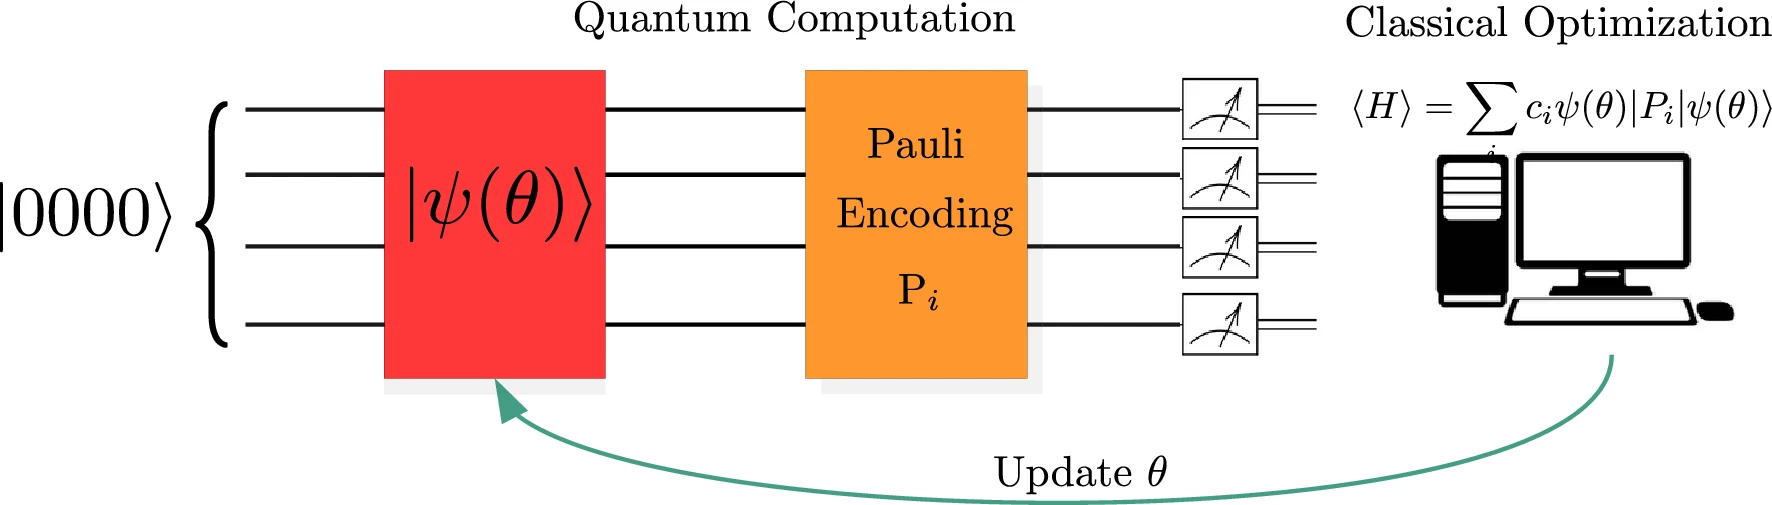
\includegraphics[width=0.9\textwidth]{images/vqe.png}
    \caption{Schema del funzionamento del Variational Quantum Eigensolver~\cite{buonaiuto2023best}.}
    \label{fig:circuitoVQE}
\end{figure}




\subsection{Quantum Approximate Optimization Algorithm}\label{sec:qaoa}
Il Quantum Approximate Optimization Algorithm (QAOA) è un algoritmo variazionale 
quantistico progettato per trovare soluzioni approssimate a problemi di 
ottimizzazione combinatoria. Il suo funzionamento si basa sull'alternanza di 
due operatori: un operatore di \textit{costo} e un operatore di \textit{mixing}, 
il quale quest'ultimo ha il compito di esplorare lo spazio delle soluzioni.

L'algoritmo opera attraverso una sequenza di strati (\textit{layers}) quantistici, 
dove ogni strato è composto da due parti principali:

\begin{equation}
   \hat{U}_C(\gamma) = e^{-i\gamma \hat{H}_C} \quad \text{(operatore di costo)},
\end{equation}
\begin{equation}    
   \hat{U}_M(\beta) = e^{-i\beta \hat{H}_M} \quad \text{(operatore di mixing)},
\end{equation}

dove $\hat{H}_C$ è l'Hamiltoniano di costo che codifica il problema da ottimizzare, 
e $\hat{H}_M$ è l'Hamiltoniano di mixing che permette di esplorare lo spazio delle 
soluzioni. I parametri $\gamma$ e $\beta$ sono parametri variazionali che vengono 
ottimizzati durante l'esecuzione dell'algoritmo.

Il circuito quantistico inizia preparando tutti i qubit nello stato di sovrapposizione:

\begin{equation}
   |s\rangle = |+\rangle^{\otimes n} = \frac{1}{\sqrt{2^n}}\sum_{x\in\{{0,1\}}^n} |x\rangle.
\end{equation}

Lo stato finale dopo $p$ layers è dato da:

\begin{equation}
   |\psi_p(\gamma, \beta)\rangle = e^{-i\beta_p \hat{H}_M} e^{-i\gamma_p \hat{H}_C} \cdots e^{-i\beta_1 \hat{H}_M} e^{-i\gamma_1 \hat{H}_C} |s\rangle
\end{equation}

L'obiettivo è massimizzare il valore atteso dell'Hamiltoniano di costo:

\begin{equation}
   F_p(\gamma, \beta) = \langle\psi_p(\gamma, \beta)| \hat{H}_C |\psi_p(\gamma, \beta)\rangle
\end{equation}

Il processo di ottimizzazione avviene in modo ibrido: il circuito quantistico prepara e 
misura gli stati, mentre un ottimizzatore classico aggiorna i parametri $\gamma$ e $\beta$ 
per massimizzare $F_p$. Questo processo viene ripetuto fino a quando non si trova una 
soluzione soddisfacente al problema di ottimizzazione (Figura~\ref{fig:circuitoQAOA}).

L'algoritmo QAOA rappresenta quindi un ponte tra il calcolo quantistico e quello classico, 
sfruttando i vantaggi di entrambi i paradigmi per risolvere problemi di ottimizzazione 
complessi. La sua efficacia dipende dal numero di layer $p$ utilizzati e dalla qualità 
dell'ottimizzazione dei parametri.


\begin{figure}[h!]
    \centering
    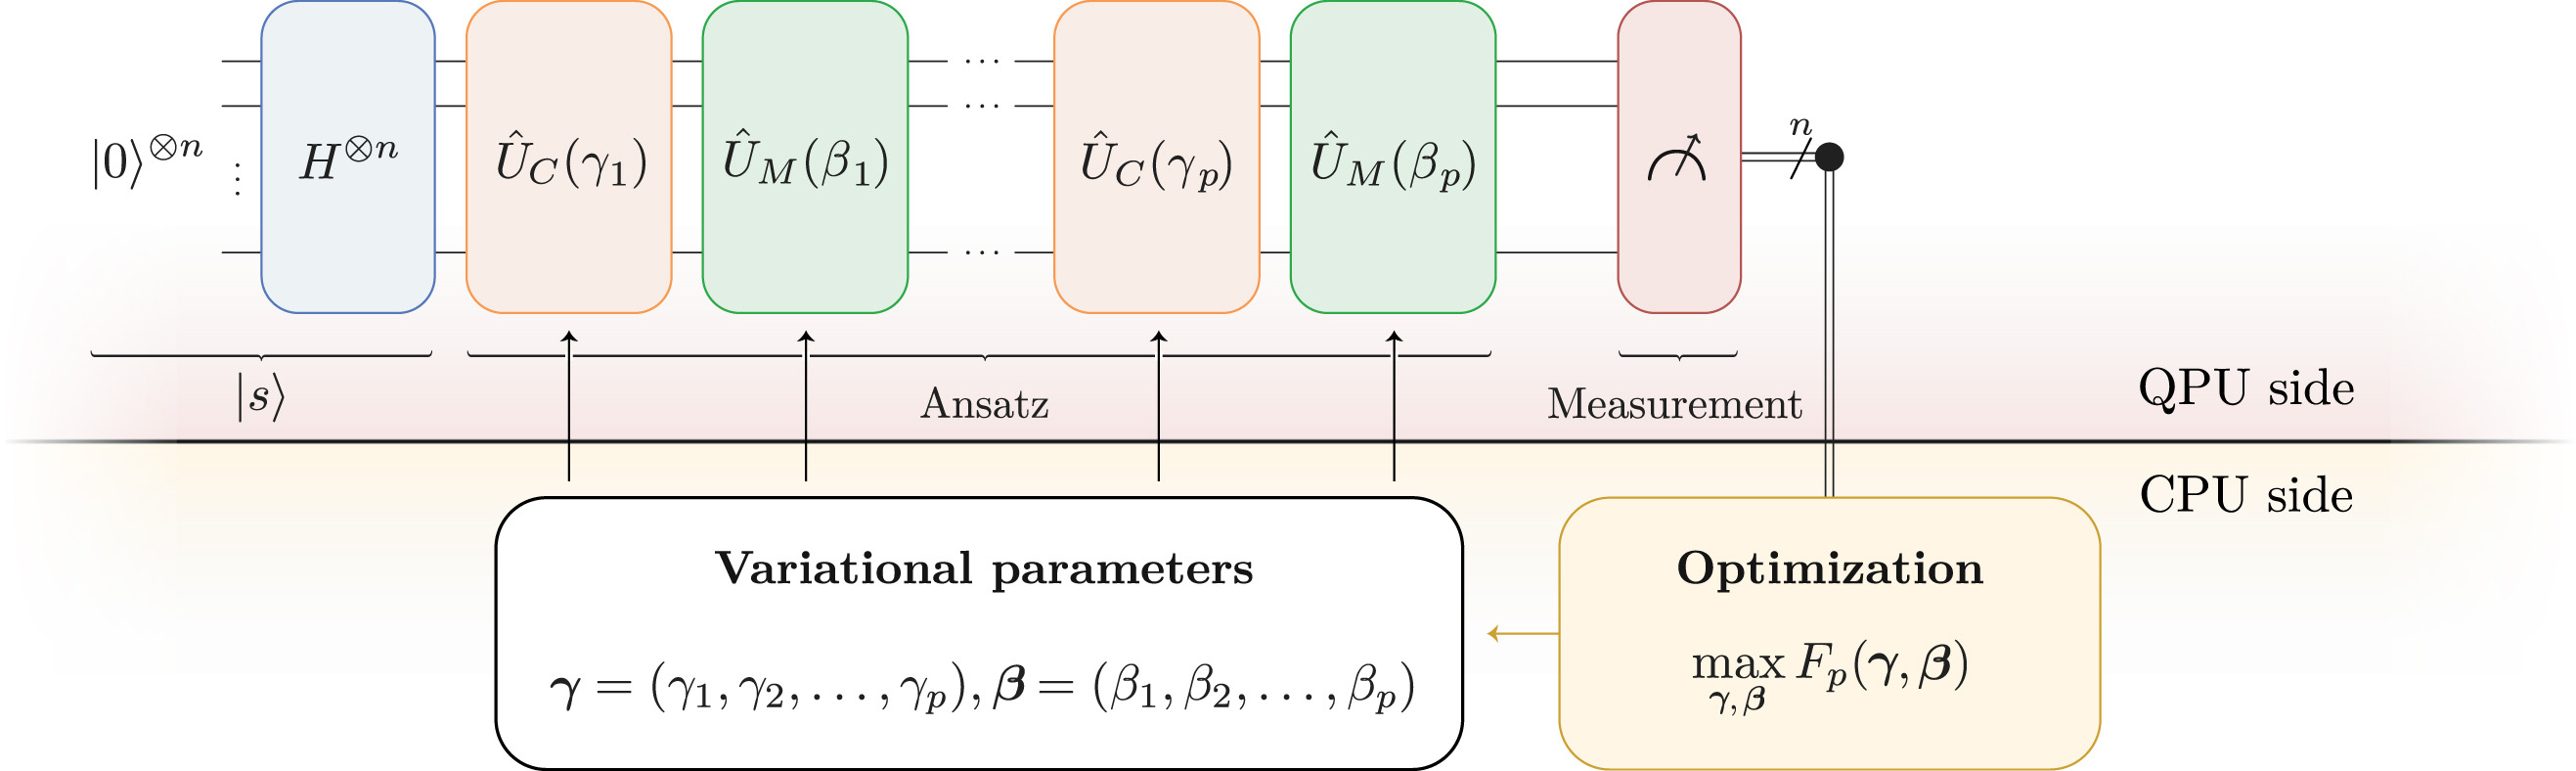
\includegraphics[width=0.9\textwidth]{images/qaoa.jpg}
    \caption{Schema del funzionamento del Quantum Approximate Optimization Algorithm~\cite{blekos2024review}.}
    \label{fig:circuitoQAOA}
\end{figure}